% !TeX spellcheck = ru_RU

% В данной главе описывается реализация компонентов решения...

\subsection{Алгоритм выделения семантического вектора}
План:
\begin{enumerate}
\item 
Для выделения семантического вектора, соответствующего редактируемому признаку, в латентном пространстве сети, в данном решении реализуется алгоритм InterFaceGAN.

\item 
Рассмотрим произвольный бинарный семантический признак, заданный дискриминативной функцией $\theta : \mathcal X \mapsto [0,1]$, характеризующей наличие или отсутствие этого признака на изображении. 
В данной работе в качестве такой функции $\theta$ используется нейросетевой классификатор, обученный на наборе данных CelebA-HQ \cite{liu2015celeba, progressive-growing-gan} предсказанию лицевых атрибутов.
В качестве архитектуры крассификатора взята архитектуре дискриминатора, используемого в \cite{progressive-growing-gan, StyleGAN}. 
В качестве рассматриваемых признаков были выбраны \emph{наличие улыбки} и \emph{поворот головы}.

\item 
Наличие такого классификатора позволяет автоматически сгенерировать два набора латентных векторов, первый из которых содержит латентные вектора, соответствующие изображениям, на которых присутствует рассматриваемый признак, второй --- отсутствует.
Для этого из латентного пространства $\mathcal W$ сэмплируется набор из $200000$ случайных латентных векторов $\mathbf w_j$, с помощью которых генератором сети StyleGAN генерируется $200000$ синтетических изображений.
Сгенерированные изображения подаются на вход классификатору $\theta$, затем данный набор латентных векторов сортируется по возрастанию полученного значения $ y_j = \theta(G(\mathbf w_j))$, которое характеризует уверенность классификатора в том, что на изображениии присутствует рассматриваемый признак.
В качестве первого набора выбирается $10000$ латентных векторов с наибольшим значением, что соответствует изображениям, на которых признак присутствует с наибольшей уверенностью.
В качестве второго --- $10000$ латентных векторов с наименьшим значением, что соответствует изображениям, на которых признак отсутствует с наибольшей уверенностью.

\item 
Поскольку два данных набора латентных векторов будут линейно разделимы в латентном пространстве, как показано в \cite{StyleGAN}, нахождение семантического вектора рассматриваемого признака сводится к нахождению оптимальной раздиляющей гиперплоскости. 
Для этого на полученном наборе векторов обучается линейная SVM \cite{svm}.
В качестве семантического вектора используется нормальный вектор найденной гиперплоскости (рис. \ref{fig:svm-boundary}).

\begin{figure}[h]
\begin{center}
    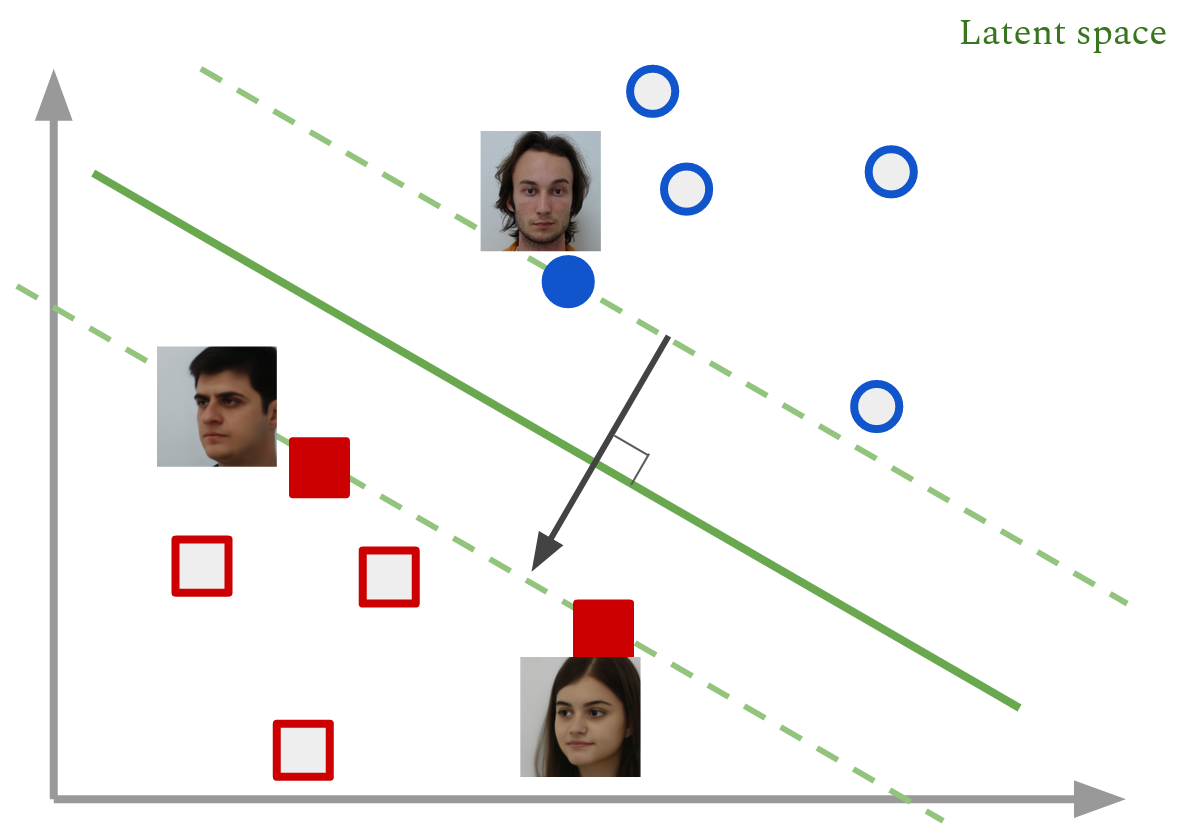
\includegraphics[width=0.7\textwidth]{boundary-SVM}
    \caption{Иллюстрация процесса нахождения семантических векторов, соответствующих отдельным факторам вариации, путем нахожения оптимальной разделяющей гиперплоскости.}
    \label{fig:svm-boundary}
\end{center}
\end{figure}

\end{enumerate}

\subsection{Предсказание начального приближения латентной оптимизации}
План:
\begin{enumerate}
% предобработка: даунскейл до 256

\item 
% Для реконструкции входных изображений ...
В качестве энкодера, используемого для предсказания начального приближения латентной оптимизации, была обучена сверточная нейронная сеть ResNet \cite{he2016resnet}.

\item 
Обучение сети производилось на наборе пар <\emph{изображение, вектор}>, составленном из $50000$ синтетических изображений, сгенерированных генеративной состязательной сетью StyleGAN, и соответствующих им входных векторов из расширенного латентного пространства $\mathcal W+$, предстваляющих собой конкатенацию 18 латентных векторов $\mathbf w_i \in \mathbb R^{512}$.
Задачей обучаемого энкодера является регрессия латентного вектора по заданному входному изображению.

\item 
В качестве функции потерь использован логарифм гиперболического синуса ошибки (\emph{Log-Cosh Loss}) между предсказанным и реальным латентными ректорами. Эта функция является гладким аналогом средней абсолютной ошибки, который дает более качественные результаты в задаче регрессии латентных векторов \cite{chen2019log}.

\item 
Нейронная сеть реализована на фреймворке PyTorch. Сеть обучалать $20$ эпох методом обратного распространения ошибки с использованием оптимизационного алгоритма Adam \cite{kingma2014adam}.

%график?

\end{enumerate}

\subsection{Нейросетевая архитектура латентной оптимизации}
План:
\begin{enumerate}
% предобработка: центрирование, апскейл до 1024
% постобработка: блюр

\item 
Для улучшения полученного приближения латентного вектора применяется алгоритм латентной оптимизации. Он позволяет приблизить латентный вектор путем минимизации функции потерь реконструкции.

\item 
В качестве функцию потерь реконструкции используется взвешенная сумма среднеквадратичной ошибки в пространстве пикселей и визуальной функции потерь (\emph{perceptual loss} \cite{Johnson2016Perceptual}).
% MSE/MAE? ... в пр-ве признаков, извлеченных VGG.
% Это позволяет не застревать в лок. мин., при этом оптимизировать RGB

\begin{figure}[h]
\begin{center}
    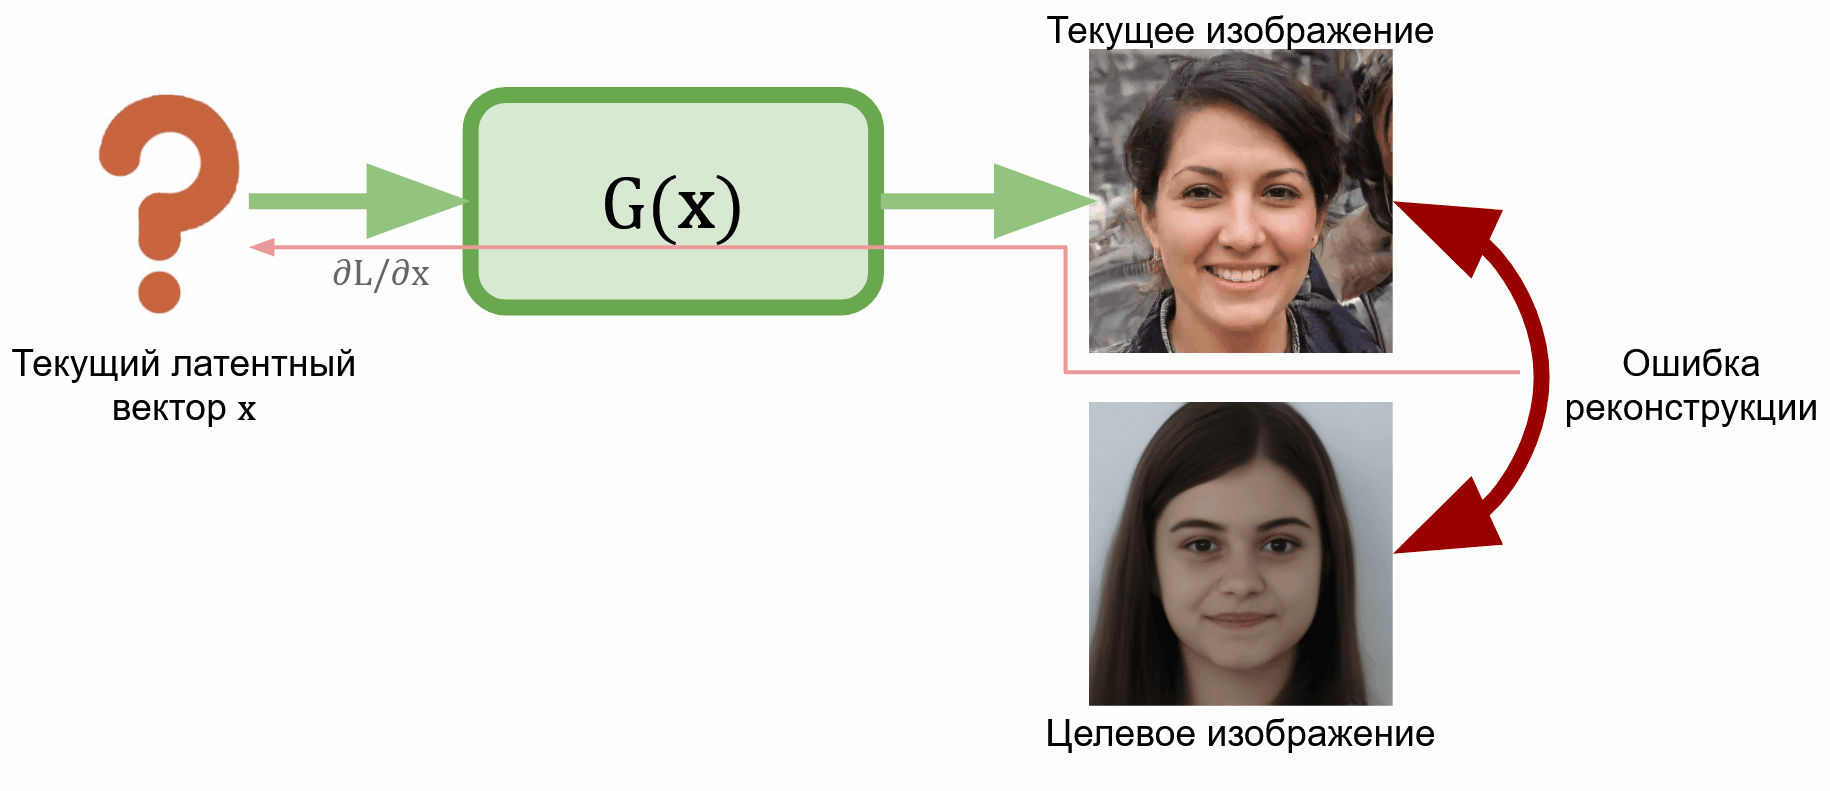
\includegraphics[width=0.9\textwidth]{optim_pipeline_ru}
    \caption{Нейросетевая архитектура латентной оптимизации}
    \label{fig:optim_pipeline}
\end{center}
\end{figure}

\item 
Минимизация функции потерь реконструкции производится путем итеративного обновления латентного вектора с помощью метода градиентного спуска (рис. \ref{fig:optim_pipeline}).
Текущий латентный вектор подается на вход генератору сети StyleGAN.
По сгенерированному изображению и целевому изображению вычисляется значение функции потерь реконструкции. Метод обратного распространения ошибки позволяет распространить градиент через генератор, тем самым получив значение градиента функции потерь по входному вектору. Затем производится шаг градиентного спуска и обновление текущего латентного вектора.
Процесс латентной оптимизации останавливается по достижении максимального количества итераций.

%\item 
%Оптимизация латентного вектора производится в расширенном пространстве $\mathcal W+$.
%Регуляризаци оптимизации, которая предназначена для предотвращения попадания в плохо определенные области латентного пр-ва (см. Latent Space Oddity), производится путем обновления только первых k мапов на первых итерациях.
% (это технический момент, который наверно не стоит включать в текст если он не будет подкреплен экспериментальными данными).

\item 
Оптимизация производится с использованием фреймворка PyTorch, для ускорения сходимости используется оптимизационный алгоритм Adam.

\end{enumerate}

\subsection{Алгоритм переноса лицевых признаков с изображения образца}
План:
\begin{enumerate}
\item
Для семантического редактирования изображений к латентным векторам, полученным в ходе реконструкции этих изображений, применяется линейный сдвиг в направлении смантического вектора редактируемого признака.

\item
Пусть $\mathbf b$ --- семантический вектор, найденный с помощью алгоритма InterFaceGAN, а $\mathbf w$ --- латентный вектор, соответствующий входному изображению.
Тогда на сгенерированном изображении $G(\mathbf w + \lambda \mathbf b)$, полученном путем линейного сдвига, рассматриваемый семантический признак будет более выражен при $\lambda > 0$, и менее выражен при $\lambda  < 0$.
Для определения величины сдвига $\lambda$ используется латентный вектор $\mathbf w_{exemplar}$, полученный в ходе реконструкции изображения-образца. 
Величина линейного сдвига будет равна расстоянию между проекциями обоих латентных векторов на $\mathbf b$: 
$$\lambda = \langle \mathbf w_{exemplar}, \mathbf b \rangle - \langle \mathbf w, \mathbf b \rangle .$$

\item
В связи с запутанностью латентного пространства, линейный сдвиг в направлении семантического вектора рассматриваемого признака может привести к измененнию других признаков. 
В частности, это может привести к изменению семантических признаков, которые определяют личность изображенного человека. 
В таком случае лицо на изображении, полученном в результате редактирования, не будет соответствовать лицу на оригинальном изображении.

\item
Чтобы этого избежать, производится модификация алгоритма. 
Задача редактирования семантического признака формулируется в виде задачи минимизации следующей функции потерь переноса
\begin{align*}
\min_{\mathbf w} &L(\mathbf w) = L_{feature}(\mathbf w, \mathbf w_{exemplar}) + \alpha~L_{identity}(\mathbf w, I_{real}), \\
&L_{feature}(\mathbf w, \mathbf w_{exemplar}) = \lvert \langle \mathbf w_{exemplar}, \mathbf b \rangle - \langle \mathbf w, \mathbf b \rangle \rvert,\\
&L_{identity}(\mathbf w, I_{real}) = - \langle f(I_{real}), f(G(\mathbf w)) \rangle.
\end{align*}
Член $L_{feature}$ отвечает за минимизацию расстояния между проекциями латентных векторов целевого изображения $\mathbf w$ и изображения-образца $\mathbf w_{exemplar}$ на семантический вектор $\mathbf b$.

Член $L_{identity}$ отвечает за сохранение личностных признаков между оригинальным и отредактированным изображениями. Для этого данным членом производится максимизация меры косинусного сходства (\emph{cosine similarity}) между эмбеддингами оригинального и отредактированного изображения, полученными с помощью модели для распознавания лиц $f$.
В качестве модели для распознавания лиц $f$ используется нейронная сеть ArcFace \cite{deng2018arcface}.

\item
Для минимизации функции потерь переноса предлагается попеременно минимизировать член $L_{feature}$ и член $L_{identity}$:
\begin{itemize}
    \item Производится фиксированный шаг в направлении семантического вектора
    $$\mathbf w'_i = \mathbf w_i + \lambda \mathbf b, \quad \lambda = \frac{\langle \mathbf w_{exemplar}, \mathbf b \rangle - \langle \mathbf w, \mathbf b \rangle}{N}.$$
    \item По изображению, сгенерированному с помощью полученного латентного вектора, вычисляется эмбеддинг и сравнивается с эмбеддингом изображения-образца для вычисления значения
    $L_{identity} = - \langle f(I_{real}), f(G(\mathbf w'_i)) \rangle.$
    \item С помощью метода обратного распространения ошибки градиент распространяется через генератор, и производится шаг градиентного спуска.
    Для исключения влияния этого шага на редактируемый признак, полученные градиенты проецируются на гиперплоскость, для которой вектор $\mathbf b$ является нормальным.
    \begin{align*}
    &\mathbf g = \frac{\partial L_{identity}}{\partial \mathbf w'_i} - \left\langle {\frac{\partial L_{identity}}{\partial \mathbf w'_i} , \mathbf b} \right\rangle \cdot \mathbf b,\\
    &\mathbf w_{i+1} = \mathbf w'_i - \alpha \mathbf g.
    \end{align*}
\end{itemize}

Процесс минимизации останавливается по достижении максимального количества итераций $N$, когда расстояние между проекциями латентных векторов входного изображения и изображения-образца на семантический вектор редактируемого признака становится равным нулю.

\item
Оптимизация производится с использованием фреймворка PyTorch.

\end{enumerate}